%%%%%%%%%%%%%%%%%%%%%%%%%%%%%%%%%%%%%%%%%
% Beamer Presentation
% LaTeX Template
% Version 1.0 (10/11/12)
%
% This template has been downloaded from:
% http://www.LaTeXTemplates.com
%
% License:
% CC BY-NC-SA 3.0 (http://creativecommons.org/licenses/by-nc-sa/3.0/)
%
%%%%%%%%%%%%%%%%%%%%%%%%%%%%%%%%%%%%%%%%%

%----------------------------------------------------------------------------------------
%	PACKAGES AND THEMES
%----------------------------------------------------------------------------------------

\documentclass[14pt]{beamer}

\mode<presentation> {

% The Beamer class slide themes
\usetheme{Madrid} %i was using this one

% Beamer class color themes

%\usecolortheme{albatross}

%\setbeamertemplate{footline} % To remove the footer line in all slides uncomment this line
%\setbeamertemplate{footline}[page number] % To replace the footer line in all slides with a simple slide count uncomment this line

%\setbeamertemplate{navigation symbols}{} % To remove the navigation symbols from the bottom of all slides uncomment this line
}

\usepackage{graphicx} % Allows including images
\usepackage{booktabs} % Allows the use of \toprule, \midrule and \bottomrule in tables
\usepackage{hyperref}
\usepackage{helvet}

%----------------------------------------------------------------------------------------
%	TITLE PAGE
%----------------------------------------------------------------------------------------

\title[bash \& SLURM]{More bash \& SLURM} % The short title appears at the bottom of every slide, the full title is only on the title page

\author{C. Ryan Campbell} % Your name
\institute[Duke] % Your institution as it will appear on the bottom of every slide, may be shorthand to save space
{
Duke University \\ % Your institution for the title page
\medskip
\textit{c.ryan.campbell@duke.edu} % Your email address
}
\date{19 Sept 2017} % Date, can be changed to a custom date

\begin{document}

\begin{frame}
\titlepage % Print the title page as the first slide
\end{frame}

\begin{frame}
\frametitle{Overview} % Table of contents slide, comment this block out to remove it
\tableofcontents % Throughout your presentation, if you choose to use \section{} and \subsection{} commands, these will automatically be printed on this slide as an overview of your presentation
\end{frame}

%----------------------------------------------------------------------------------------
%	PRESENTATION SLIDES
%----------------------------------------------------------------------------------------

%------------------------------------------------
\section{Goals} % A subsection can be created just before a set of slides with a common theme to further break down your presentation into chunks
%------------------------------------------------

%------------------------------------------------
\begin{frame}
\frametitle{Today's Goals}
\begin{itemize}
	\item<+-> Log into the cluster
	\item<+-> Learn some basic commands
	\begin{itemize}
		\item<+-> sort, uniq, cut, nano
	\end{itemize}
	\item<+-> Learn some advanced commands
	\begin{itemize}
		\item<+-> grep, sed, awk
	\end{itemize}
	\item<+-> Answer some Emmy trivia questions
\end{itemize}
\end{frame}

%------------------------------------------------
\section{Cluster Basics}
%------------------------------------------------

%------------------------------------------------
\begin{frame}
\frametitle{More Twitter}
	\begin{center}
     	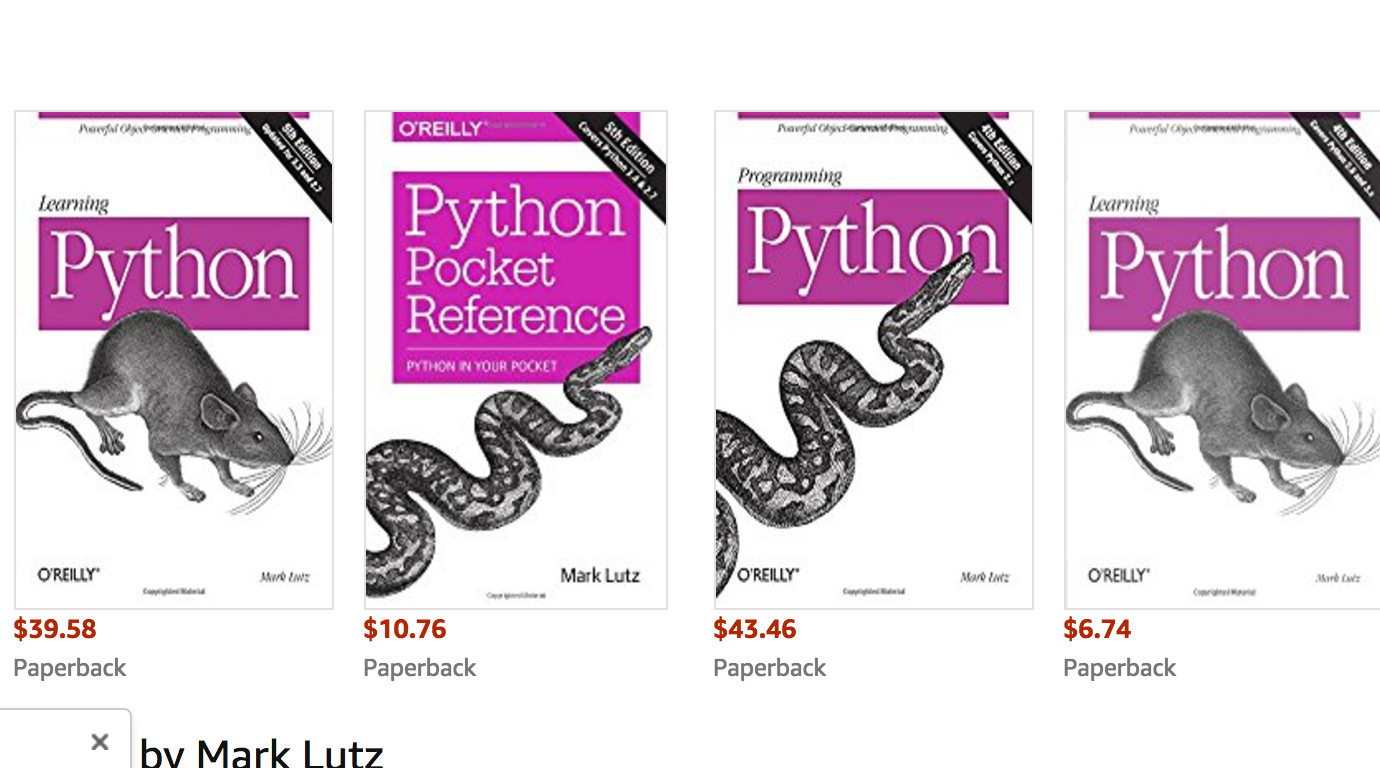
\includegraphics[width=1\textwidth]{images_20170919_python.png}
    \end{center}
\end{frame}

%------------------------------------------------
\begin{frame}
\frametitle{More Twitter}
	\begin{center}
     	
\includegraphics[width=.6\textwidth]{images_20170919_twitter.png}
    \end{center}
\end{frame}

%------------------------------------------------
\subsection{Recap}
%------------------------------------------------

%------------------------------------------------
\begin{frame}
\frametitle{Logging On}
\begin{itemize}
	\item Use command ``ssh''
	\item Logs on to one of two compute nodes:
	\ttfamily
	\begin{block}{}
		\item[] ssh <netid>@dscr-slogin-01.oit.duke.edu
	\end{block}
	\sffamily
	\item Your terminal window is now on the computer ``dscr-slogin-01.oit.duke.edu''
	\item You may have set up an alias:
	\ttfamily
	\footnotesize
	\begin{block}{}
		\item[] alias DSCR="ssh <your netid>@dscr-slogin-01.oit.duke.edu"
	\end{block}
\end{itemize}
\end{frame}

%------------------------------------------------
\begin{frame}
\frametitle{File Generation}
\begin{itemize}
	\item nano - text-based text editor
	\item<+-> Adding a filename ``\texttt{nano <file>}'' opens that file
	\item[]
	\item<+-> Or make a file on your local computer
	\item And use \texttt{scp} to move it up to the cluster
\end{itemize}
\end{frame}

%------------------------------------------------
\begin{frame}
\frametitle{Tips and Help}
\begin{itemize}
	\item Spaces and order matter
	\item General grammar rules:
	\item[] \texttt{<command> <flags> <input>}
	\item If you're unsure what the flags are ``-h'' or ``--help'' often works
	\item Using ``tab'' auto-completes filenames and commands
	\item Prevents typos
\end{itemize}
\end{frame}

%------------------------------------------------
\begin{frame}
\frametitle{You Ran a Cluster Script!}
\begin{itemize}
	\item<+-> Ta-Da!! Now you can run a job on the cluster!
	\item<+-> You now have the minimum knowledge to get onto the cluster and use the resource to run software that is unsuitable for your laptop
	\item<+-> Now, there are a lot more things that the cluster and bash can do, mostly involving data manipulation
	\item<+-> Let's delve into some of those!
\end{itemize}
\end{frame}

%------------------------------------------------
\begin{frame}
\frametitle{Datafile}
\begin{itemize}
	\item Emmy Winners 1949 to Present
	\small
	\item[] \texttt{/work/cc216/490S/cc216/emmy-awards-1949-2017.csv}
	\normalsize
	\item Copy to your own folder, then pull out the nominees
	\small
	\begin{block}{}
		\item[] \texttt{grep \textasciicircum20.., emmy-awards-1949-2017.csv | sed 's/, Nonfiction,//g' | cut -d, -f4 > nominees.list}
		\tiny
		\item[]
		\item[] \texttt{grep \textasciicircum20.., emmy-awards-1949-2017.csv | sed 's/, Nonfiction,//g' | cut -d, -f4 > nominees.list}
	\end{block}
\end{itemize}
\end{frame}

%------------------------------------------------
\subsection{Basic Tools}
%------------------------------------------------

%------------------------------------------------
\begin{frame}
\frametitle{Tools}
\begin{itemize}
	\item Input and output from commandline
	\begin{itemize}
		\item Using \texttt{>} and \texttt{|}
	\end{itemize}
	\sffamily
	\item \texttt{cat, less, head, tail} - inspecting files and output
	\item \texttt{sort} - sorting
	\item \texttt{uniq} - sort and eliminate duplicates
	\item \texttt{cut} - split a file into columns
\end{itemize}
\end{frame}

%------------------------------------------------
\begin{frame}
\frametitle{Input and Output}
\begin{itemize}
	\item Unless otherwise noted:
	\begin{itemize}
		\item Input comes after the command
		\item Output ``prints to screen''
	\end{itemize}
	\item Using \texttt{>} and \texttt{|} changes that
	\item \texttt{>} takes output and (over)writes to a file
	\ttfamily
	\begin{block}{}
		\item[] ls > list.txt
	\end{block}
	\sffamily
	\normalsize
	\item If you use double \texttt{>>} it appends to a file
	\ttfamily
	\begin{block}{}
		\item[] ls -lt >> list.txt
	\end{block}
\end{itemize}
\end{frame}

%------------------------------------------------
\begin{frame}
\frametitle{Input and Output}
\begin{itemize}
	\item Using \texttt{|} changes input
	\item \texttt{|} takes output and passes it to the next command
	\ttfamily
	\begin{block}{}
		\item[] ls | head -n1
	\end{block}
	\sffamily
	\normalsize
	\item You can string together many \texttt{|}'s to perform complicated actions
\end{itemize}
\end{frame}

%------------------------------------------------
\begin{frame}
\frametitle{Inspecting Files and Output}
\begin{itemize}
	\item \texttt{cat, less, head, tail}
	\item \texttt{cat} - prints the whole file to screen
	\ttfamily
	\begin{block}{}
		\item[] cat <name of file>
	\end{block}
	\item \texttt{less} - opens the file so you can scroll through it (q to quit)
	\sffamily
	\normalsize
	\item \texttt{head, tail} - return the first or last 10 lines of a file
	\ttfamily
	\begin{block}{}
		\item[] head <name of file>; tail <name of file>
	\end{block}
	\sffamily
	\item Common flags:
	\begin{itemize}
		\item -n number of lines (overrides 10)
	\end{itemize}
\end{itemize}
\end{frame}

%------------------------------------------------
\begin{frame}
\frametitle{sort}
\begin{itemize}
	\item \texttt{sort} takes input and sorts it! (simple, right?)
	\ttfamily
	\begin{block}{}
		\item[] sort <name of file>
		\item[] cat <name of file> | sort 
	\end{block}
	\sffamily
	\normalsize
	\item Common flags:
	\begin{itemize}
		\item -n sorts numerically
		\item -u sorts and only presents unique hits
		\item -r sorts reverse
		\item -t, and -k sort the nth field (k), separated by ,
	\end{itemize}
\end{itemize}
\end{frame}

%------------------------------------------------
\begin{frame}
\frametitle{uniq}
\begin{itemize}
	\item \texttt{uniq} takes input and removes adjacent duplicates! (still simple, right?)
	\ttfamily
	\begin{block}{}
		\item[] uniq <name of file>
		\item[] cat <name of file> | uniq 
	\end{block}
	\sffamily
	\normalsize
	\item Common flags:
	\begin{itemize}
		\item -c counts each unique line
		\item -d reverses the meaning (prints only duplicates)
	\end{itemize}
\end{itemize}
\end{frame}

%------------------------------------------------
\begin{frame}
\frametitle{cut}
\begin{itemize}
	\item \texttt{cut} takes input and divides it into ``columns''
	\ttfamily
	\begin{block}{}
		\item[] cut -d<what to divide by> -f<which columns you want> <name of file>
	\end{block}
	\sffamily
	\normalsize
	\item Common flags:
	\begin{itemize}
		\item -d what to divide by (``,'' `` '' ``tab'')
		\item -c take n characters (-c1-10 takes first 10 characters in each line)
		\item -f which columns you want:
		\begin{itemize}
			\item -f1, first only
			\item -f1-5 one through five
			\item -f1,5 first and fifth only
		\end{itemize}
	\end{itemize}
\end{itemize}
\end{frame}

%------------------------------------------------
\subsection{Advanced Tools}
%------------------------------------------------

%------------------------------------------------
\begin{frame}
\frametitle{Advanced Tools}
\begin{itemize}
	\item The following tools are more advanced and complicated
	\item You will often see them in online forums
	\item You don't have to be a wizard
	\item It is good to be familiar with them
	\scriptsize
	\item[] (Once you are, there isn't a dataset you won't be able to manage)
	\normalsize
	\item \texttt{grep} - regular expression search
	\item \texttt{sed} - search and replace patterns
	\item \texttt{awk} - counting as well as search
\end{itemize}
\end{frame}

%------------------------------------------------
\begin{frame}
\frametitle{grep}
\begin{itemize}
	\item \texttt{grep} searches, line by line, for a pattern or ``regular expression''
	\item Globally search a Regular Expression and Print
	\ttfamily
	\begin{block}{}
		\item[] grep <pattern to find> <name of file>
	\end{block}
	\sffamily
	\normalsize
	\item Common flags:
	\begin{itemize}
		\item -i case-independent
		\item -v reverse-search (all lines WITHOUT the pattern)
		\item -c returns a count instead of the lines
		\item -w surround the pattern with whitespace
		\item -A or -B return pattern and n-lines after (A) or before (B) 
	\end{itemize}
\end{itemize}
\end{frame}

%------------------------------------------------
\begin{frame}
\frametitle{sed}
\begin{itemize}
	\item \texttt{sed} searches and replaces a pattern
	\item Prints result to screen
	\ttfamily
	\begin{block}{}
		\item[] sed `s,<old pattern>,<new pattern>,g' <name of file>
	\end{block}
	\sffamily
	\normalsize
	\item Common flags:
	\begin{itemize}
		\item -i in-place, replaces the pattern in the file and overwrites
		\item -i.bak in-place, same as above but saves the initial as originalfilename.bak
	\end{itemize}
\end{itemize}
\end{frame}

%------------------------------------------------
\begin{frame}
\frametitle{awk}
\begin{itemize}
	\item \texttt{awk} is very powerful and mysterious
	\item If I'm using it, it is likely from a google search
	\item To find the average of the second column:
	\ttfamily
	\begin{block}{}
		\item[] cat <name of file> | awk '{ sum += \$2 } END { if (NR > 0) print sum / NR }'
	\end{block}
	\sffamily
	\item ``Add up column 2, if more than 1 row then print the sum divided by the rows''
	\item Great for advanced math (bash can, generally, only handle integers)
\end{itemize}
\end{frame}

%------------------------------------------------
\subsection{Revisting the Datafile}
%------------------------------------------------

%------------------------------------------------
\begin{frame}
\frametitle{Revisiting the Datafile}
\begin{itemize}
	\item Emmy Winners 1949 to Present
	\item What did these commands do?
	\small
	\begin{block}{}
		\item[] \texttt{grep \textasciicircum20.., emmy-awards-1949-2017.csv | sed 's/, Nonfiction,//g' | cut -d, -f4 > nominees.list}
		\tiny
	\end{block}
	\normalsize
	\item[] grep - 
	\item[] \texttt{|} - 
	\item[] sed - 
	\item[] cut - 
	\item[] \texttt{>} - 
\end{itemize}
\end{frame}

%------------------------------------------------
\begin{frame}
\frametitle{Revisiting the Datafile}
\begin{itemize}
	\small
	\item<+-> \texttt{grep \textasciicircum20.., emmy-awards-1949-2017.csv | sed 's/, Nonfiction,//g' | cut -d, -f4 > nominees.list}
	\item<+-> grep - search for 20\#\#, in the Emmys file
	\item<+-> \texttt{|} - take output and feed it to sed
	\item<+-> sed - replace ", Nonfiction," with ""
	\item<+-> cut - pull out the 4th column, by commas
	\item<+-> \texttt{>} - write to file named nominees.list
\end{itemize}
\end{frame}

%------------------------------------------------
\begin{frame}
\frametitle{Revisiting the Datafile}
\begin{itemize}
	\Large
	\item[] Answer the following:
	\normalsize
	\item[] How many Emmys was Netflix nominated for in 2015?
	\item[] How many different shows?
	\item[] Which show had the most?
	\item[] How many Emmys has GoT been nominated for?
\end{itemize}
\end{frame}

%------------------------------------------------
\begin{frame}
\frametitle{Revisiting the Datafile}
\begin{itemize}
	\Large
	\item[] Answer the following:
	\normalsize
	\item[] How many Emmys was Netflix nominated for in 2015? (15)
	\item[] How many different shows? (7)
	\item[] Which show had the most? (House of Cards - 6)
	\item[] How many Emmys has GoT been nominated for? (105)
\end{itemize}
\end{frame}


%------------------------------------------------
\begin{frame}
\Huge{\centerline{The End}}
\end{frame}

%----------------------------------------------------------------------------------------

\end{document} 